\section{相关工作概述}
\label{related}

《奶牛营养需要》第7版(NRC 2011)\footnote{该手册有中文版,百度搜索其中文名称即可找到、下载。}\cite{USA2001Nutrient}中,第一章讨论奶牛的干物质采食量(Dry Matter Intake,DMI)。下文引自《奶牛营养需要》中文版原文。

用来预测荷斯坦泌乳牛DMI的方程式为:
\begin{eqnarray}
\label{eqn:dmi}
	 \nonumber DMI (kg/d) =&&(0.372  \times FCM \\
	 \nonumber &&+  0.0968 \times  BW^{0.75}) \\
	&&\times (1 - e^{-0.192 \times(WOL + 3.67)})
\end{eqnarray}
式中FCM=4\%校正乳产量(kg/d);BW=体重(kg);WOL为泌乳周龄;$1-e^{-0.192\times(WOL+3.67)}$为校正泌乳早期DMI下降的校正项。对于泌乳早期的产奶牛来说,方程式1-2预测的结果与Kertz等(1991)所建立方程式的预测结果相一致。最初14周龄泌乳牛干物质采食量以不同方程式预测的比较结果列于图\ref{fig:dmi}。

\begin{figure}
\begin{center}
	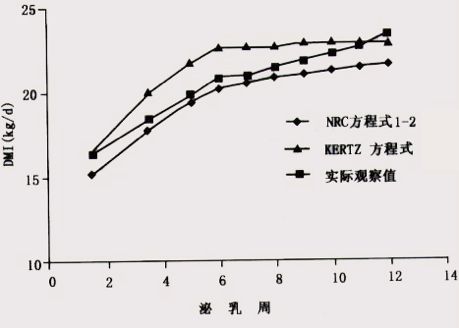
\includegraphics[width=0.9\linewidth]{dmi}
\caption{用方程式\ref{eqn:dmi}和KERTZ等(1991)推荐方程式预测奶牛泌乳早期干物质采食量变化。(图中方程式1-2对应本文中方程式1。)}
\label{fig:dmi}
\end{center}
\end{figure}

方程式\ref{eqn:dmi}的数据全部来自荷斯坦奶牛。目前还没有公开发表关于DMI的数据用于发展或修正目前预测DMI的方程式,以便能用在荷斯坦牛以外其他品种牛上。关于娟姗牛DMI的预测问题,请参见Holter等(1996)的文章。

DMI预测方程式用于经产奶牛可不必进行校正。
在热中温区(5$\sim$20℃)以外,泌乳牛的DMI受到环境的影响。Eastridge等(1998)和Holter等(1997)的研究都表明,当环境温度在20℃以上时,DMI随温度的升高而下降。由于没有足够的数据来确定热中温区以外环境对DMI的影响程度,本版NRC泌乳牛DMI预测方程式(方程式\ref{eqn:dmi})没有考虑温度或湿度校正因子。